\iflong
\begin{figure}[hpt!]
\else
\begin{wrapfigure}[]{r}{.4\textwidth}
\fi
\centering
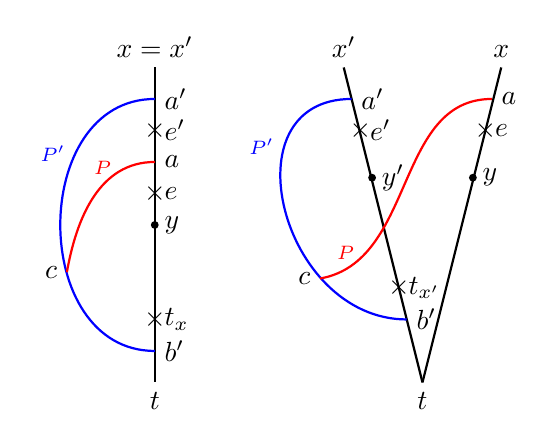
\begin{tikzpicture}[scale=2]

\definecolor{dgreen}{rgb}{0.0, 0.5, 0.0}
\begin{scope}[xshift=0cm]
\coordinate (s) at (0,2);
\coordinate (t) at (0,0);
\coordinate (ts) at (0,0.4);
\coordinate (b1) at (0,.2);
\coordinate (y) at (0,1);
\coordinate (a1) at (0,1.8);
\coordinate (a) at (0,1.4);
\coordinate (v) at (0,1.2);
\coordinate (v1) at (0,1.6);
\coordinate (c) at (-0.558,0.7);

\draw[thick](s)--(t);
\node[above] at (s){$x=x'$};
\node[below] at (t){$t$};
\node[right] at (a1){$a'$};
\node[right] at (a){$a$};
\node[right] at (b1){$b'$};
\node[left] at (c){$c$};


\draw[blue,thick] (a1) to[out=180,in=180,distance=.8cm]
node[pos=0.3,left]
{\scriptsize  $P'$}  (b1);

\draw[red,thick] (a) to[out=180,in=80]
node[pos=0.4,above]
{\scriptsize  $P$}  (c);

\node at (v1){$\times$};
\node[right] at (v1){$e'$};

\node at (v){$\times$};
\node[right] at (v){$e$};

\node at (ts){$\times$};
\node[right] at (ts){$t_x$};

\draw (y) node[fill,circle,scale=0.3]{};
\node[right] at (y){$y$};

\end{scope}

\begin{scope}[xshift=1.7cm]
\coordinate (s) at (-0.5,2);
\coordinate (s1) at (0.5,2);

\coordinate (t) at (0,0);
\coordinate (ts) at (-0.15,0.6);
\coordinate (b1) at (-0.1,0.4);
\coordinate (y1) at (-0.32,1.3);
\coordinate (y) at (0.32,1.3);
\coordinate (a1) at (-0.45,1.8);
\coordinate (a) at (0.44,1.8);
\coordinate (v) at (0.4,1.6);
\coordinate (v1) at (-0.395,1.6);
\coordinate (c) at (-0.65,0.66);

\draw[thick](s)--(t);
\draw[thick](s1)--(t);
\node[above] at (s){$x'$};
\node[above] at (s1){$x$};
\node[below] at (t){$t$};
\node[right] at (a1){$a'$};
\node[right] at (a){$a$};
\node[right] at (b1){$b'$};
\node[left] at (c){$c$};


\draw[blue,thick] (a1) to[out=180,in=180,distance=.8cm]
node[pos=0.3,left]
{\scriptsize  $P'$}  (b1);

\draw[red,thick] (a) to[out=180,in=10]
node[pos=0.9,above]
{\scriptsize  $P$}  (c);

\node at (v1){$\times$};
\node[right] at (v1){$e'$};

\node at (v){$\times$};
\node[right] at (v){$e$};

\node at (ts){$\times$};
\node[right] at (ts){$t_{x'}$};

\draw (y1) node[fill,circle,scale=0.3]{};
\node[right] at (y1){$y'$};

\draw (y) node[fill,circle,scale=0.3]{};
\node[right] at (y){$y$};

\end{scope}






\end{tikzpicture}

\caption{The figure shows two representative examples when $ca$ and $at$ does not pass through $e'$.}
\label{fig:examples}
\iflong
\end{figure}
\else
\end{wrapfigure}
\fi
